
\documentclass[11pt]{article}
\usepackage[margin=1in]{geometry}

%packages
\usepackage{graphicx}
\usepackage{hyperref}
\usepackage{amssymb}

\begin{document}

\title{\textbf{ md2tex }}
\author{ Pratik Shrestha }
\maketitle

\section{Title 1}

Following are some examples from md2tex.

\subsection{Bold and Italics}

This is an example of \textbf{bold} and this for \textit{italics}. This is an example \textbf{\textit{both}}.

\subsection{Lists}

\subsubsection{Ordered}
\begin{enumerate}
    \item item 1
    \item item 2
    \item item 3
    \item item 4
\end{enumerate}

\subsubsection{Unordered}
\begin{itemize}
    \item item 1
    \item item 2
    \item item 3
    \item item 4
\end{itemize}

\subsection{Table}

\begin{tabular}{|l|l|l|}
\hline
Header 1&Header 2&Header 3 \\
\hline
a&b&c \\
d&e&f \\
\hline
\end{tabular}

\subsection{Image}

\begin{figure}
\centering
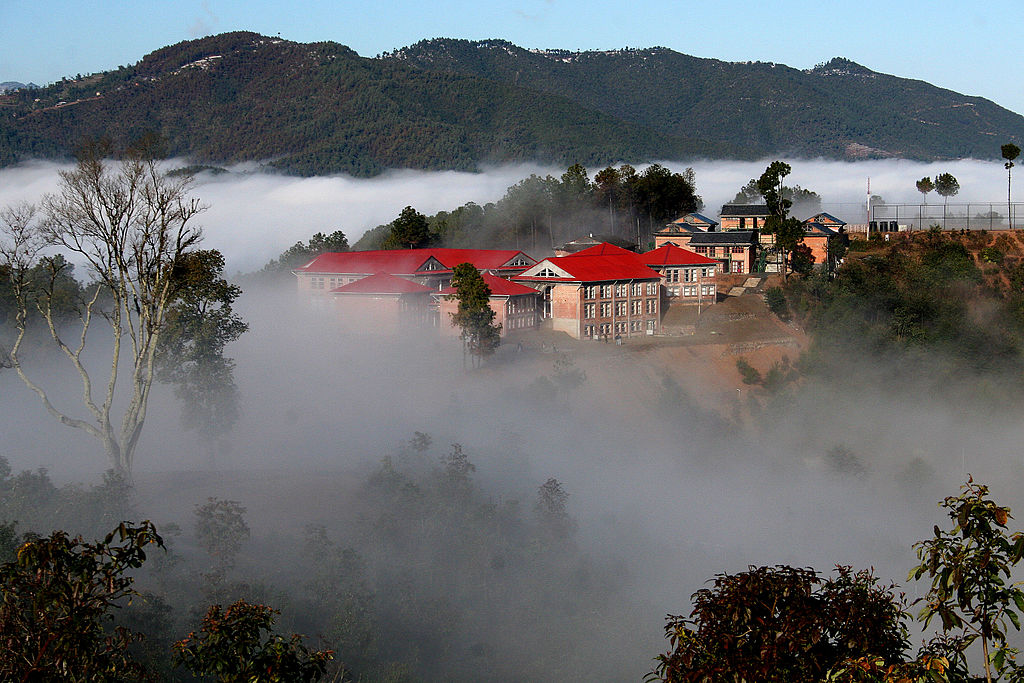
\includegraphics[width=\textwidth]{sample.jpg}
\end{figure}
\begin{figure}
\centering
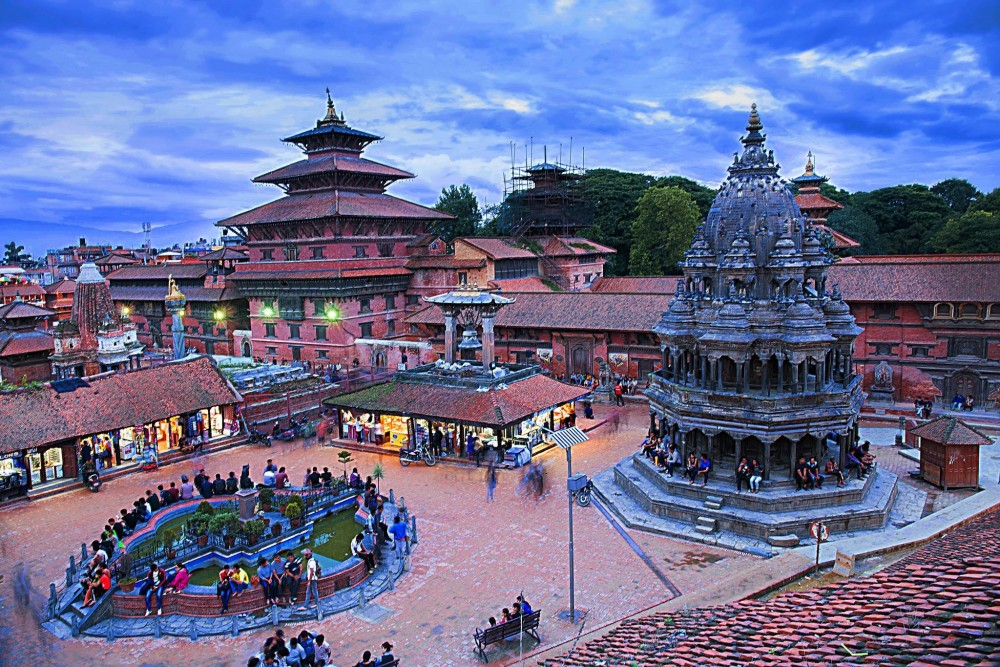
\includegraphics[width=\textwidth]{sample2.jpeg}
\caption{Sample}
\end{figure}

\subsection{Links}

You can catch me on twitter \href{https://twitter.com/prtxpratik}{@prtxpratik}


\end{document}